\documentclass{article}
\usepackage{amsmath, sfmath, multicol, tkz-euclide, array, enumerate, tcolorbox, tabularray, tipa}
\renewcommand{\familydefault}{\sfdefault}
\setlength{\parindent}{0cm}
\pagestyle{empty}
\usepackage[left=1in, top=0.5in, right=1in, bottom=0.5in]{geometry}
\tikzset{>=stealth, label style/.append style={font=\footnotesize}}
\tcbset{colback=white}

\newcounter{example}[section]
\newenvironment{example}[1][]{\refstepcounter{example}\par\medskip
   {\color{red}\textbf{Example~\theexample. #1}}}{\medskip}

\newcommand{\arc}[1]{%
    \setbox9=\hbox{#1}%
    \ooalign{\resizebox{\wd9}{\height}{\texttoptiebar{\phantom{A}}}\cr#1}}

\begin{document}

\section*{Tangent Lines}

\begin{tcolorbox}[colframe=orange!70!white, coltitle=black, title=\textbf{Today I Can}]
\begin{enumerate}
    \item Use properties of a tangent to a circle.
\end{enumerate}
\end{tcolorbox}
\smallskip 

\begin{tcolorbox}[colframe=black!20!white, opacitybacktitle=0.1, coltitle=black, title=\textbf{Tangent Line}]
A line that intersects a circle at only one point (the \textit{point of tangency}). \newline 

\begin{minipage}{0.5\textwidth}
    \begin{itemize}
        \item $\overleftrightarrow{AB}$ is \textbf{tangent} to $\odot O$.
        \item $P$ is the \textbf{point of tangency}.
    \end{itemize}
\end{minipage}
\begin{minipage}{0.4\textwidth}
    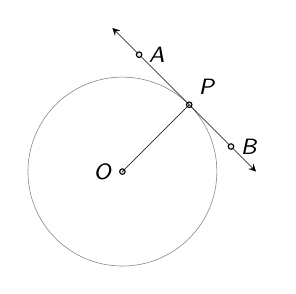
\begin{tikzpicture}[scale=0.6]
    \tkzDefPoints{0/0/O}
    \tkzDefShiftPoint[O](45:2){P}
    \tkzDrawCircle(O,P)
    \tkzLabelPoints[left](O)
    \tkzDrawPoints(O,P)
    \tkzDrawSegment(O,P)
    \tkzDefLine[orthogonal=through P](O,P)    \tkzGetPoint{h}
    \tkzDrawSegment[add=1 and 0.15, <->, >=stealth](P,h)
    \tkzDefShiftPoint[P](135:1.5){A}
    \tkzDrawPoint(A)
    \tkzDefShiftPoint[P](-45:1.25){B}
    \tkzDrawPoint(B)
    \tkzLabelPoints[right](A,B)
    \tkzLabelPoints[above right](P)
    \end{tikzpicture}
\end{minipage}
\end{tcolorbox}
\bigskip 

\begin{example}
$\overline{ML}$ and $\overline{MN}$ are tangent to $\odot O$. What is the value of $x$? \newline

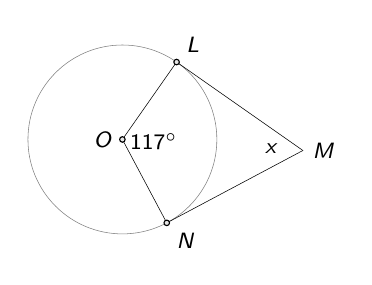
\begin{tikzpicture}[scale=0.8]
\tkzDefPoints{0/0/O}
\tkzDefShiftPoint[O](55:1.5){L}
\tkzDefShiftPoint[O](-62:1.5){N}
\tkzDrawCircle(O,L)
\tkzDefLine[orthogonal=through L](O,L) \tkzGetPoint{e}
\tkzDefLine[orthogonal=through N](O,N) \tkzGetPoint{f}
\tkzInterLL(L,e)(N,f)   \tkzGetPoint{M}
\tkzDrawSegments(L,M N,M O,L O,N)
\tkzDrawPoints(O,L,N)
\tkzLabelPoints[left](O)
\tkzLabelPoints[right](M)
\tkzLabelPoints[above right](L)
\tkzLabelPoints[below right](N)
\tkzLabelAngle[pos=0.5](L,M,f){\footnotesize $x$}
\tkzLabelAngle[pos=0.5](N,O,L){\footnotesize $117^\circ$}
\end{tikzpicture}
\end{example}

\vfill 

\begin{example}
Find the length of the unknown segments.
\begin{multicols}{2}
\begin{enumerate}[(a)]
    \item \mbox{}
    \item \mbox{}
\end{enumerate}
\end{multicols}
\begin{minipage}{0.5\textwidth}
    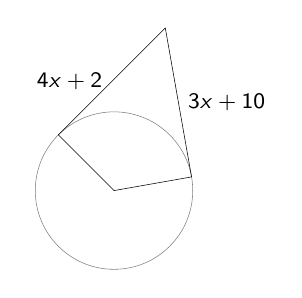
\begin{tikzpicture}
    \tkzDefPoints{0/0/O}
    \tkzDefShiftPoint[O](10:1){A}
    \tkzDefShiftPoint[O](135:1){C}
    \tkzDrawCircle(O,A)
    \tkzDrawSegments(O,C O,A)
    \tkzDefLine[orthogonal=through A](O,A) \tkzGetPoint{d}
    \tkzDefLine[orthogonal=through C](O,C) \tkzGetPoint{e}
    \tkzInterLL(A,d)(C,e)   \tkzGetPoint{B}
    \tkzDrawSegments(B,C B,A)
    \tkzLabelSegment[left](B,C){$4x+2$}
    \tkzLabelSegment[right](B,A){$3x+10$}
    \end{tikzpicture}
\end{minipage}
\begin{minipage}{0.4\textwidth}
    \begin{tikzpicture}
    \tkzDefPoints{0/0/O, 2/0/A, -2/0/B}
    \tkzDrawPoint(O)
    \tkzDrawCircle(O,A)
    \tkzGetPoint{a}
    \tkzDrawSegments(A,B)
    \draw (2,-2) -- (-2,0);
    \tkzLabelSegment[above](O,B){7.5}
    \node at (2,-1) [anchor = west] {?};
    \draw [|<->|, >=stealth, xshift=-0.15cm, yshift=-0.15cm] (-2,0) -- (2,-2);
    \draw (A) -- (2,-2);
    \node at (-0.25,-1.15) [anchor = north] {17};
    \end{tikzpicture}
\end{minipage}
\end{example}

\vfill 
\newpage 

\begin{example}
Find the perimeter of each polygon.
\begin{multicols}{2}
\begin{enumerate}[(a)]
    \item \mbox{} 
    \item \mbox{}
\end{enumerate}
\end{multicols}
\begin{minipage}{0.5\textwidth}
    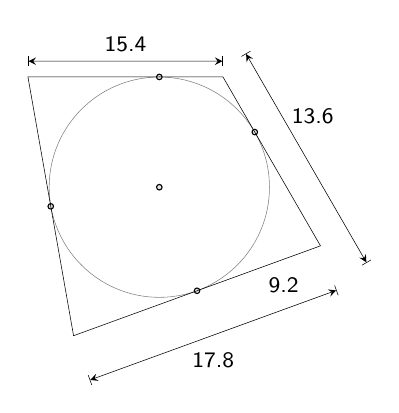
\begin{tikzpicture}[scale=0.8]
    \tkzDefPoints{0/0/O}
    \tkzDefShiftPoint[O](30:1.75){A}
    \tkzDrawCircle(O,A)
    \tkzDefShiftPoint[O](90:1.75){B}
    \tkzDefShiftPoint[O](190:1.75){C}
    \tkzDefShiftPoint[O](290:1.75){D}
    \tkzDrawPoints(A,B,C,D,O)
    % \tkzLabelPoints(A,B,C,D,O)
    \tkzDefLine[orthogonal = through A](O,A)  \tkzGetPoint{a}
    \tkzDefLine[orthogonal = through B](O,B)  \tkzGetPoint{b}
    \tkzDefLine[orthogonal = through C](O,C)  \tkzGetPoint{c}
    \tkzDefLine[orthogonal = through D](O,D)  \tkzGetPoint{d}
    \tkzInterLL(A,a)(B,b)   \tkzGetPoint{z}
    \tkzInterLL(B,b)(C,c)   \tkzGetPoint{y}
    \tkzInterLL(C,c)(D,d)   \tkzGetPoint{x}
    \tkzInterLL(D,d)(A,a)   \tkzGetPoint{w}
    \tkzDrawSegments(A,z B,z B,y C,y C,x D,x A,w D,w)
    \tkzLabelSegment[below right](D,w){9.2}
    \tkzDefShiftPoint[O](290:2.5){E}
    \tkzDefLine[parallel=through E](w,x)    \tkzGetPoint{e}
    \tkzDrawSegment[|<->|, >=stealth, add=0.5 and -0.5](E,e)
    \tkzLabelPoint[below,yshift=-0.1cm](E){17.8}
    \tkzDefShiftPoint[O](30:2.25){F}
    \tkzDefLine[parallel=through F](a,w)    \tkzGetPoint{f}
    \tkzDrawSegment[|<->|, >=stealth, add = 0.3 and -0.3](F,f)
    \tkzLabelPoint[right](F){13.6}
    \tkzDefShiftPoint[O](90:2.25){G}
    \tkzDefLine[parallel=through G](b,y)    \tkzGetPoint{g}
    \tkzDefShiftPoint[y](0,0.25){y'}
    \tkzDefShiftPoint[z](0,0.25){z'}
    \tkzDrawSegment[|<->|, >=stealth](y',z')
    \tkzLabelSegment[above](y',z'){15.4}
    \end{tikzpicture}
\end{minipage}
\begin{minipage}{0.4\textwidth}
    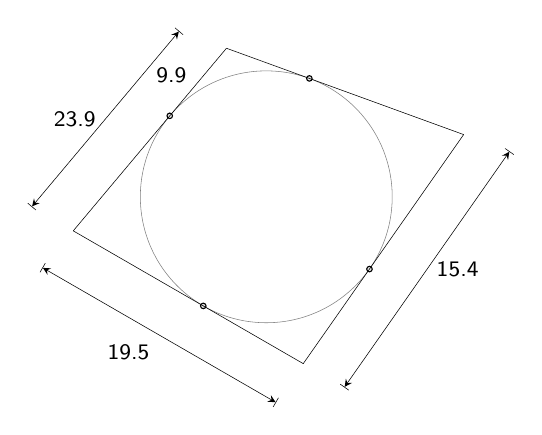
\begin{tikzpicture}[scale=0.8]
    \tkzDefPoints{0/0/O}
    \tkzDefShiftPoint[O](70:2){A}
    \tkzDefShiftPoint[O](140:2){B}
    \tkzDefShiftPoint[O](240:2){C}
    \tkzDefShiftPoint[O](325:2){D}
    \tkzDrawCircle(O,A)
    \tkzDrawPoints(A,B,C,D)
    \tkzDefLine[orthogonal = through A](O,A)    \tkzGetPoint{a}
    \tkzDefLine[orthogonal = through B](O,B)    \tkzGetPoint{b}
    \tkzDefLine[orthogonal = through C](O,C)    \tkzGetPoint{c}
    \tkzDefLine[orthogonal = through D](O,D)    \tkzGetPoint{d}
    \tkzInterLL(A,a)(B,b)   \tkzGetPoint{z}
    \tkzInterLL(B,b)(C,c)   \tkzGetPoint{y}
    \tkzInterLL(C,c)(D,d)   \tkzGetPoint{x}
    \tkzInterLL(D,d)(A,a)   \tkzGetPoint{w}
    \tkzDrawSegments(A,z B,z B,y C,y C,x D,x A,w D,w)
    \tkzLabelSegment[left, xshift=0.2cm](a,B){9.9}
    \tkzDefShiftPoint[O](140:2.75){E}
    \tkzDefShiftPoint[O](240:2.75){F}
    \tkzDefShiftPoint[O](325:2.75){G}
    \tkzDefLine[parallel = through E](z,y)  \tkzGetPoint{e}
    \tkzInterLL(A,z)(E,e)   \tkzGetPoint{e'}
    \tkzInterLL(C,y)(E,e)   \tkzGetPoint{y'}
    \tkzDrawSegment[|<->|, >=stealth](e',y')
    \tkzLabelSegment[left](e',y'){23.9}
    \tkzDefLine[parallel = through F](x,y)  \tkzGetPoint{f}
    \tkzInterLL(z,y)(F,f)   \tkzGetPoint{f'}
    \tkzDefLine[parallel = through G](x,w)  \tkzGetPoint{g}
    \tkzInterLL(f',F)(w,x)   \tkzGetPoint{r'}
    \tkzDrawSegment[|<->|, >=stealth](f',r')
    \tkzLabelSegment[below left](f',r'){19.5}
    \tkzInterLL(G,g)(w,z)   \tkzGetPoint{h}
    \tkzInterLL(h,g)(x,y) \tkzGetPoint{i}
    \tkzDrawSegment[|<->|](h,i)
    \tkzLabelSegment[right](h,i){15.4}
    \end{tikzpicture}
\end{minipage}
\end{example}


\end{document}
